\documentclass[aspectratio=169]{beamer}
\usetheme{Boadilla}
\useoutertheme{infolines}
\setbeamertemplate{navigation symbols}{}

\usepackage{fontspec}
\usepackage{unicode-math}
\usepackage[Latin,Greek]{ucharclasses}
\usepackage{amsmath}
\usepackage{stmaryrd}
\usepackage{newunicodechar}
\usepackage{proof}
\usepackage[conor,links]{agda}
\usepackage[backend=biber]{biblatex}
\addbibresource{references.bib}
\usepackage{tikz}
\usetikzlibrary{cd}
\usepackage{adjustbox}

\definecolor{bblue}{rgb}{0.2,0.2,0.7}

\makeatletter
\def\th@remarkstyle{
    \normalfont
    \setbeamercolor{block title example}{bg=orange!40,fg=orange}
    \setbeamercolor{block body example}{bg=orange!20,fg=black}
    \def\inserttheoremblockenv{exampleblock}
  }
\makeatother
\theoremstyle{remarkstyle}
\newtheorem*{remark}{Remark}

\newunicodechar{ƛ}{\ensuremath{\lambda}}
\newunicodechar{ℕ}{\ensuremath{\mathbb{N}}}
\newunicodechar{⋅}{\ensuremath{\cdot}}


\title{From De Bruijn to co-De Bruijn using Category Theory}
\subtitle{Everybody's Got To Be Somewhere$^{\text{\cite{codebruijn}}}$}
\institute[Uni Freiburg]{Chair of Programming Languages, University of
  Freiburg}
\author{Marius Weidner}

\begin{document}

\begin{frame}
  \titlepage{}
\end{frame}

\begin{frame}{Outline}
  \tableofcontents
\end{frame}

\section{Getting Started: Scopes and Binders Categorically}
\subsection{The Category of Scopes}

\begin{frame}[fragile]
  \frametitle{The Category of Scopes: $Δ_+^X$}
  \begin{definition}
    Let $Δ_+^X$ be the category of scopes with
    \begin{itemize}
      \item Objects: $\bar{x}, \bar{y}, \bar{s} ∈ |Δ_+^X| = X^*$ and
      \item Morphisms: $f, g ∈ Δ_+^X(\bar{x}, \bar{y})$ for $\bar{x}, \bar{y} ∈ X^*$ are inductively defined by inference rules
    \end{itemize}
    \begin{columns}
      \begin{column}{0.04\textwidth}
      \end{column}
      \begin{column}{0.2\textwidth}
        \begin{center}
          \infer[·]{
            ε ⊑ ε
          }{}
        \end{center}
      \end{column}
      \begin{column}{0.2\textwidth}
        \begin{center}
          \infer[1]{
            \bar{x}x ⊑ \bar{y}x
          }{
            \bar{x} ⊑ \bar{y}
          }
        \end{center}
      \end{column}
      \begin{column}{0.2\textwidth}
        \begin{center}
          \infer[0]{
            \bar{x} ⊑ \bar{y}y
          }{
            \bar{x} ⊑ \ \bar{y}
          }
        \end{center}
      \end{column}
      \begin{column}{0.3\textwidth}
      \end{column}
    \end{columns}
  \end{definition}
  % \begin{corollary}
  %   The initial object of the $Δ_+^X$ category is the empty scope $ε$ with the $\bar{0}$ as the unique morphism. 
  % \end{corollary}
  \begin{remark}
    Morphisms in $Δ_+^X$ can be represented by \emph{bit vectors} $\bar{b} ∈ \{0, 1\}^*$ with one bit per variable of the target scope telling whether it has been mapped to or skipped by the source scope.
  \end{remark}
\end{frame}

\begin{frame}[fragile]
  \frametitle{Objects \& Morphisms in $Δ_+^⊤$}
  \begin{example}
    Let $X = ⊤$, where $⊤$ is the set with exactly one element $⟨⟩$.\\ Then, objects in $Δ_+^⊤$ represent numbers. 
    \begin{columns}
      \begin{column}{0.6\textwidth}
        \begin{center}
          \adjustbox{scale=0.6}{
            \begin{tikzcd}
              3 \arrow[rr, "10101"]  &         & 5 &   &   &   &   &   &   \\
                                     &         &   &   &   &   &   &   &   \\
              • \arrow[rr, no head]  &         & • &   &   &   &   &   & 1 \\
                                     &         & ∘ &   &   &   &   & 0 &   \\
              • \arrow[rr, no head]  &         & • &   &   &   & 1 &   &   \\
                                     &         & ∘ &   &   & 0 &   &   &   \\
              • \arrow[rr, no head]  &         & • &   & 1 &   &   &   &   \\
                                     &         &   & · &   &   &   &   &  
            \end{tikzcd}
          }
        \end{center}
      \end{column}
      \begin{column}{0.4\textwidth}
        \begin{center}
          \adjustbox{scale=1.3}{
            \begin{tikzcd}
              3 \arrow[d, "10101"', bend right] \arrow[d, dashed, bend left] \arrow[rd, dotted, bend left] \arrow[d, dashed, bend left=60] &    \\
              5                                                                                                                             & {}
            \end{tikzcd}
          }
        \end{center}
      \end{column}
    \end{columns}
  \end{example}
\end{frame}

\begin{frame}[fragile]
  \frametitle{Identity and Composition in $Δ_+^⊤$}
  \begin{columns}
    \begin{column}{0.20\textwidth}
      \begin{example}
        \begin{center}
          \adjustbox{scale=0.8}{
            \begin{tikzcd}
              5 \arrow[rr, "id" = 11111]    &  & 5 \\
                                    &  &   \\
              • \arrow[rr, no head] &  & • \\
              • \arrow[rr, no head] &  & • \\
              • \arrow[rr, no head] &  & • \\
              • \arrow[rr, no head] &  & • \\
              • \arrow[rr, no head] &  & • 
            \end{tikzcd}
          }
        \end{center}
      \end{example}
    \end{column}
    \begin{column}{0.75\textwidth}
      \begin{example}
        \adjustbox{scale=0.8}{
          \begin{tikzcd}
            2 \arrow[rr, "101"]  &  & 3 &  & 3 \arrow[rr, "10101"]&  & 5 &  & 2 \arrow[rr, "10001"]   &  & 5 \\
                                  &  &   &  &                       &  &   &  &                       &  &   \\
            • \arrow[rr, no head] &  & • &  & • \arrow[rr, no head] &  & • &  & • \arrow[rr, no head] &  & • \\
                                  &  &   &  &                       &  & ∘ &  &                       &  & ∘ \\
                                  &  & ∘ & ; & • \arrow[rr, no head] &  & • & =  &                       &  & ∘ \\
                                  &  &   &  &                       &  & ∘ &  &                       &  & ∘ \\
            • \arrow[rr, no head] &  & • &  & • \arrow[rr, no head] &  & • &  & • \arrow[rr, no head] &  & •
          \end{tikzcd}
        }
      \end{example}
    \end{column}
  \end{columns}
\end{frame}

\begin{frame}[fragile]
  \frametitle{$Δ_+^X$ is in Fact a Category}
  \begin{columns}
    \begin{column}{0.33\textwidth}
      % \Large{\color{bblue} $Δ_+^X$ is in Fact a Category}
      \begin{lemma}
        \begin{small}
          In $Δ_+^X$ every object $\bar{x} ∈ X^*$ has an identity morphism, 
          i.e. we can construct an identity morphism for every object $\bar{x}$ using the inference rules.
        \end{small}
      \end{lemma}
      \begin{proof}
        \begin{small}
        $id \ \ \ \ \ \ : \ \bar{x} ⊑ \bar{x}$\\
        $id \ ε \ \ \ = \ ·$\\
        $id \ \bar{x} x \ = \ id 1$
        \end{small}
      \end{proof}
      \begin{corollary}
        \begin{small}
        $id-l \ \, : \ id ; f = f$ \\
        $id-r \ : \ f;id = f$
        \end{small}
      \end{corollary}  
    \end{column}
    \begin{column}{0.62\textwidth}
      \begin{definition}
        
        In $Δ_+^X$ two morphisms $f : \bar{x} ⊑ \bar{y}$ and $g : \bar{y} ⊑ \bar{z}$ 
        compose to a morphism $f;g : \bar{x} ⊑ \bar{z}$, 
        i.e. we can construct a morphism $f;g$ from $f$ and $g$ using the inference rules:

        \vspace{8mm}

        $\_;\_ \ \ \ \ \ \ : \ \bar{x} ⊑ \bar{y} → \bar{y} ⊑ \bar{z} → \bar{x} ⊑ \bar{z}$\\
        $·  \ \ \, ; \ · \ \ \ \ = \ ·$\\
        $f 1  \ ; \ g 1 \ = \ (f;g)1$\\
        $f 0 \ ; \ g 1  \ = \ (f;g)0$\\
        $f \ \ \, ; \ g 0 \ = \ (f;g)0$
        
      \end{definition}
      \begin{corollary}
        \begin{small}
        assoc \ \ \ \ : \ $f;(g;h) = (f;g);h$\\
        antisym \ : \ $(f : \bar{x} ⊑ \bar{y}) → (g : \bar{y} ⊑ \bar{x}) → \bar{x} = \bar{y} \land f = g = id \ \bar{x}$
        \end{small}
      \end{corollary}  
    \end{column}
  \end{columns}
\end{frame}


\subsection{Intrinsically Scoped De Bruijn Syntax}

\begin{frame}[fragile]
  \frametitle{Intrinsically Scoped De Bruijn Syntax via $Δ_+^⊤$}
  \begin{definition}
    Let $Tm : ℕ → Set$ be the set of lambda calculus terms inductively defined by
    \begin{columns}
      \begin{column}{0.2\textwidth}
        \begin{center}
          \infer[\#]{
            Tm \ n
          }{
            1 ⊑ n
          }
        \end{center}
      \end{column}
      \begin{column}{0.3\textwidth}
        \begin{center}
          \infer[\$]{
            Tm \ n
          }{
            Tm \ n &  
            Tm \ n
          }
        \end{center}
      \end{column}
      \begin{column}{0.3\textwidth}
        \begin{center}
          \infer[λ]{
            Tm \ n
          }{
            Tm \ (n + 1)
          }
        \end{center}
      \end{column}
    \end{columns}
  \end{definition}
  \begin{example}
    $𝕂 = λx. λy. x \quad \quad \quad \quad \ \ = λ \ λ \ \#1$\\
    $𝕊 = λx. λy. λz. x \ z \ (y \ z) = λ \ λ \ λ \ \#2 \ \#0 \ (\#1 \ \#0)$
  \end{example}
\end{frame}

\section{Going Further: From De Bruijn to co-De Bruijn}
\subsection{The Slice Category of Subscopes}

\begin{frame}[fragile]
  \frametitle{The Slice Category of Subscopes: $Δ_+^X∖\bar{s}$}
  \begin{definition}
    \begin{columns}
      \begin{column}{0.68\textwidth}
        Let $Δ_+^X∖\bar{s}$ be the category of subscopes for a given $\bar{s} ∈ X^*$ with 
        \begin{itemize}
          \item Objects: $\bar{b}, (\bar{x}, f) ∈ |Δ_+^X∖\bar{s}| = \left(\bar{x} : X^* × Δ_+^X(\bar{x}, \bar{s}) \right)$ and
          \item Morphisms: $h ∈ [Δ_+^X∖\bar{s}]((\bar{x}, f), (\bar{y}, g))$ such that $f = h;g$ 
        \end{itemize}
      \end{column}
      \begin{column}{0.3\textwidth}
        \adjustbox{scale=1}{
          \begin{tikzcd}
            \bar{x} \arrow[rdd, "f"', dotted] \arrow[rr, "h"] &   & \bar{y} \arrow[ldd, "g", dotted] \\
                                                        &   &                            \\
                                                        & \bar{s} &                           
          \end{tikzcd}
        }
      \end{column}
    \end{columns}
  \end{definition}
  \begin{remark}
    Objects in $Δ_+^X∖\bar{s}$ can be represented by \emph{bit vectors} $\bar{b} ∈ \{0, 1\}^*$ with one bit per variable of scope $\bar{s}$, telling whether it has been selected.
  \end{remark}
\end{frame}

\begin{frame}[fragile]
  \frametitle{Objects \& Morphisms in $Δ_+^T∖5$}
  \begin{example}
    \begin{columns}
      \begin{column}{0.5\textwidth}
        \adjustbox{scale=1.5}{
          \begin{tikzcd}
            3 \arrow[rdd, "01110"', dotted] \arrow[rr, "0111"]  &   & 4 \arrow[ldd, "11110", dotted] \\
                                                                &   &                                 \\
                                                                & 5 &                                
            \end{tikzcd}
        }
      \end{column}
      \begin{column}{0.45\textwidth}
        % TODO!!!!!!!!!
        % \adjustbox{scale=0.6}{
        %   \begin{tikzcd}
        %     2 \arrow[rr, "011"]   &  & 3 &   & 3 \arrow[rr, "1110"]  &  & 4 &   & 2 \arrow[rr, "0110"]  &  & 4 \\
        %                           &  &   &   &                       &  &   &   &                       &  &   \\
        %                           &  & ∘ &   & • \arrow[rr, no head] &  & • &   &                       &  & ∘ \\
        %     • \arrow[rr, no head] &  & • &   & • \arrow[rr, no head] &  & • &   & • \arrow[rr, no head] &  & • \\
        %     • \arrow[rr, no head] &  & • & ; & • \arrow[rr, no head] &  & • & = & • \arrow[rr, no head] &  & • \\
        %                           &  &   &   &                       &  & ∘ &   &                       &  & ∘
        %   \end{tikzcd}
        % }
        Alternatively:
        \begin{itemize}
        \item \adjustbox{scale=1}{
          \begin{tikzcd}
            {(3, 01110)} \arrow[rr, "0111"] &  & {(4, 11110)}
          \end{tikzcd}
        }
        \item \adjustbox{scale=1}{
          \begin{tikzcd}
            {01110} \arrow[rr, "0111"] &  & {11110}
          \end{tikzcd}
        }
        \end{itemize}
      \end{column}
    \end{columns}
  \end{example}
\end{frame}

\begin{frame}[fragile]
  \frametitle{The Curious Case of Coproducts in $Δ_+^X∖\bar{s}$}
  \begin{theorem}
    Objects in the slice category $\bar{b}₁, \bar{b}₂ ∈ |Δ_+^X∖\bar{s}|$ have a coproduct object $\bar{b}₁ + \bar{b}₂$, i.e. there exist morphisms $l ∈ [Δ_+^X∖\bar{s}](\bar{b}₁, \bar{b}₁ + \bar{b}₂)$ and $r ∈ [Δ_+^X∖\bar{s}](\bar{b}₂, \bar{b}₁ + \bar{b}₂)$ such that every pair $f ∈ [Δ_+^X∖\bar{s}](\bar{b}₁, \bar{b}_3)$ and $g ∈ [Δ_+^X∖\bar{s}](\bar{b}₂, \bar{b}_3)$ factor through a unqiue $h ∈ [Δ_+^X∖\bar{s}](\bar{b}₁ + \bar{b}₂, \bar{b}_3)$ such that $f = l;h$ and $g = r;h$.
  \end{theorem}
  \begin{columns}
    \begin{column}{0.5\textwidth}
      \begin{example}
          \adjustbox{scale=0.76}{
            \begin{tikzcd}
              01100 \arrow[rrrrrd, "0110"] \arrow[rrd, "011"'] &  &                           &  &  &       \\
                                                               &  & 11100 \arrow[rrr, "1110"] &  &  & 11110 \\
              11000 \arrow[rrrrru, "1100"'] \arrow[rru, "110"] &  &                           &  &  &      
              \end{tikzcd}
          }
      \end{example}
    \end{column}
    \begin{column}{0.46\textwidth}
      \begin{remark}
        The coproduct $\bar{b}₁ + \bar{b}₂$ of two subscopes $\bar{b}₁, \bar{b₂}$ 
        corresponds to the minimal subscope covering both $\bar{b}₁$ and $\bar{b₂}$. 
        The coproduct $\bar{b}₁ + \bar{b}₂$ can be computed by pointwise disjunction of $\bar{b}₁$ and $\bar{b}₂$. 
      \end{remark}
    \end{column}
  \end{columns}
\end{frame}

\subsection{Sets Indexed by Scopes}

\begin{frame}[fragile]
  \frametitle{The Category $\overline{Set}$ of Sets Indexed by Scope}
  \begin{definition}
    Let $\overline{Set}$ be the category of sets indexed by scopes with
    \begin{itemize}
      \item Objects: $T, S ∈ |\overline{Set}| = \bar{X} = X^* → Set $ and 
      \item Morphisms: $f_⋅ ∈ \overline{Set}(T, S) = (\bar{x}∈X^*) → T(\bar{x}) → S(\bar{x})$
    \end{itemize}
  \end{definition}
  \begin{definition}
    Let $\_⇑\_ : \bar{X} → \bar{X} = (T, \bar{x}) ↦ (T(\bar{s}) × \bar{s} ⊑ \bar{x})$ be the set of a terms together with a selection of its variables.
    We write $t ↑ \bar{b}$ for elements of  $T ⇑ \bar{x}$. 
    % \\We define $Ref : \overline{Set} \stackrel{⋅}{→} \overline{Set}$ to be the endofunctior induced by the mapping
    % \begin{itemize}
    %   \item $Ref(T) = (\bar{x} ↦ T ⇑ \bar{x}) ∈ \bar{X}$ for objects and
    %   \item $Ref(f_⋅) = (t ↑ h) ↦ (f_⋅(t) ↑ h) ∈ T \stackrel{⋅}{→} S$ for morphisms
    % \end{itemize}
  \end{definition}
\end{frame}

% \begin{frame}[fragile]
%   \frametitle{$Δ_+^X$ makes $Ref$ a Monad!}
%   \begin{remark}
%     The set $T⇑\bar{x}$ packs an set $T ∈ \bar{X}$ indexed by $\bar{x} ∈ X^*$ applied to a subscope $\bar{s}$ of $\bar{x}$, together with a selection $h ∈ |Δ_+^X∖\bar{x}|$ of the variables of $T$.
%   \end{remark}
%   \begin{theorem}
%     The endofunctor $Ref : \overline{Set} → \overline{Set}$ gives rise to a monad with the two natural transformations
%     \begin{itemize}
%       \item $pure : Id(T) \stackrel{⋅}{→} Ref(T) = t ↦ (t ↑ id)$ and
%       \item $join : Ref(Ref(T)) \stackrel{⋅}{→} Ref(T) = ((t ↑ h₁)↑ h₂) ↦ (t ↑ h₁;h₂)$
%     \end{itemize}
%   \end{theorem}
%   \begin{example}
%     \adjustbox{scale=0.74}{
%       \begin{tikzcd}
%         Tm \arrow[rr, "pure", dashed] &  & \bar{x} ↦ (Tm \ \bar{x} ↑ \bar{x} ⊑ \bar{x}) \arrow[lld, "Ref"', dashed] \\
%         \bar{y} ↦ ([\bar{x} ↦ (Tm \ \bar{x} ↑ \bar{x} ⊑ \bar{x})] \bar{s} ↑ \bar{s} ⊑ \bar{y}) \arrow[rr, "join", dashed]  &  & \bar{y} ↦ (Tm \ \bar{s} ↑ \bar{s} ⊑ \bar{y})                        
%       \end{tikzcd}
%     }
%   \end{example}
% \end{frame}

\frametitle{The Notion of Relevant Pairs}
\begin{frame}[fragile]
  \frametitle{The Notion of Relevant Pairs}
  \begin{remark}
    The set $T⇑\bar{x}$ packs an set $T ∈ \bar{X}$ indexed by $\bar{x} ∈ X^*$ applied to a subscope $\bar{s}$ of $\bar{x}$, together with a selection $\bar{b} ∈ |Δ_+^X∖\bar{x}|$ of the variables of $T$.
  \end{remark}
  \begin{definition}
    Let $Cov : \bar{x} ⊑ \bar{s} → \bar{y} ⊑ \bar{s} → Set$ be the set of \emph{coverings} indexed by morphisms $\bar{b}₁$ and $\bar{b}₂$
    \begin{columns}
      \begin{column}{0.2\textwidth}
        \begin{center}
          \infer[·]{
            Cov \ · \ ·
          }{}
        \end{center}
      \end{column}
      \begin{column}{0.2\textwidth}
        \begin{center}
          \infer[L]{
            Cov \ \bar{b}₁1 \ \bar{b}₂
          }{
            Cov \ \bar{b}₁ \ \bar{b}₂
          }
        \end{center}
      \end{column}
      \begin{column}{0.2\textwidth}
        \begin{center}
          \infer[R]{
            Cov \ \bar{b}₁ \ \bar{b}₂1
          }{
            Cov \ \bar{b}₁ \ \bar{b}₂
          }
        \end{center}
      \end{column}
      \begin{column}{0.2\textwidth}
        \begin{center}
          \infer[B]{
            Cov \ \bar{b}₁1 \ \bar{b}₂1
          }{
            Cov \ \bar{b}₁ \ \bar{b}₂
          }
        \end{center}
      \end{column}
    \end{columns}
    Let the set of relevant pairs be defined as 
    \begin{itemize}
      \item $\_×_R\_ : \bar{X} → \bar{X} → \bar{X}  = (T, S, \bar{x}) ↦ ((\_ ↑ \bar{b}₁ : T ⇑ \bar{x}) × (\_ ↑ \bar{b}₂ : S ⇑ \bar{x}) × Cov \ \bar{b}₁ \ \bar{b}₂)$
      \item $\_,_R\_ : T ⇑ \bar{x} → S ⇑ \bar{x} → (T ×_R S) ⇑ \bar{x}$ 
      \\ \quad \quad \ $= (( t₁ ↑ \bar{b}₁), (t₂ ↑ \bar{b}₂)) ↦  ((t₁ ↑ \bar{b}₁') , (t₂ ↑ \bar{b}₂'), \bar{b}₁ ⊕ \bar{b}₂) ↑ \bar{b}'$ \\ 
    \end{itemize}
  \end{definition}
  
\end{frame}

\begin{frame}[fragile]
  \frametitle{Exploring Relevant Pairs}
  \begin{remark}
    Coverings $Cov \ \bar{b}₁ \ \bar{b}₂$ hold data about the coproduct of $\bar{b}₁$ and $\bar{b}₂$ as well as information about the original appearance of $\bar{b}₁$ and $\bar{b}₂$.
  \end{remark}
  \begin{example}
    \begin{columns}
      \begin{column}{0.56\textwidth}
          Look at $λx. λy. λz. z \ y = λ λ λ(\#0 \ \#1)$. \\
          The variable terms could also be represented as
          \begin{itemize}
            \item $z' : Tm ⇑ 3 = \#0 ↑ 001$
            \item $y' : Tm ⇑ 3 = \#1 ↑ 011$
          \end{itemize}
      \end{column}
      \begin{column}{0.44\textwidth}
          \adjustbox{scale=0.74}{
            \begin{tikzcd}
              001 \arrow[rrrrrd, "001"] \arrow[rrd, "01"'] &  &                         &  &  &     \\
                                                           &  & ⟨ BR \arrow[rrr, "011"] &  &  & 111 \\
              011 \arrow[rrrrru, "011"'] \arrow[rru, "11"] &  &                         &  &  &    
              \end{tikzcd}
          }
      \end{column}
    \end{columns}
    And the application term could be a \emph{relevant pair} 
    \begin{itemize}
     \item $z' ,_R y' : (Tm ×_R Tm) ⇑ 3 = (\#0 ↑ 01, \#1 ↑ 11, BR) ↑ 011$
    \end{itemize}
  \end{example}
\end{frame}

\subsection{Intrinsically Scoped co-De Bruijn Syntax}
\begin{frame}[fragile]
  \frametitle{Intrinsically Scoped co-De Bruijn Syntax}
  \begin{definition}
    Let $Tm : ℕ → Set$ be inductively defined: \\
    \begin{columns}
      \begin{column}{0.2\textwidth}
        \begin{center}
          \infer[\#]{
            Tm \ 1
          }{
            \\
          }
        \end{center}
      \end{column}
      \begin{column}{0.3\textwidth}
        \begin{center}
          \infer[\_,_{[\_]}\_]{
            Tm \ n
          }{
            (Tm ×_R Tm) \ n
          }
        \end{center}
      \end{column}
      \begin{column}{0.25\textwidth}
        \begin{center}
          \infer[λ]{
            Tm \ n
          }{
            Tm \ (n + 1)
          }
        \end{center}
      \end{column}
    \end{columns}
  \end{definition}
  \begin{example}
    $𝕂 = λx. λy. x \quad \quad \quad \quad \ \ = \lightning$\\
    $𝕊 = λx. λy. λz. x \ z \ (y \ z) = λ \ λ \ λ($\\
    \quad \quad $((((\# ↑ 10) ,_{[LR]} (\# ↑ 01)) ↑ 101) ,_{[LRB]} $\\
    \quad \quad $(((\# ↑ 10) ,_{[LR]} (\# ↑ 01)) ↑ 011)) ↑ id$\\
    $)$
  \end{example}
\end{frame}

\section{Wrapping Up: What I've (Not) Told You}
\subsection{This Is Actually an Agda Paper}

\begin{frame}[fragile]
  \begin{columns}
    \begin{column}{0.5\textwidth}
      \large{\color{bblue} This is actually an Agda Paper}
      \vspace{5mm}
      \begin{itemize}
        \item All categorical concepts formalized in Agda
        \item Categorical concepts applied to formally reason over programming languages using theorem provers
        \item Suitable representations of objects and morphisms that \emph{do not block} are required
        \item Comes with a \emph{universe of metasyntaxes with binding} 
        \item Defines \emph{hereditary} substitution on metasyntaxes 
      \end{itemize}
      \vspace{10mm}
    \end{column}
    \begin{column}{0.5\textwidth}
      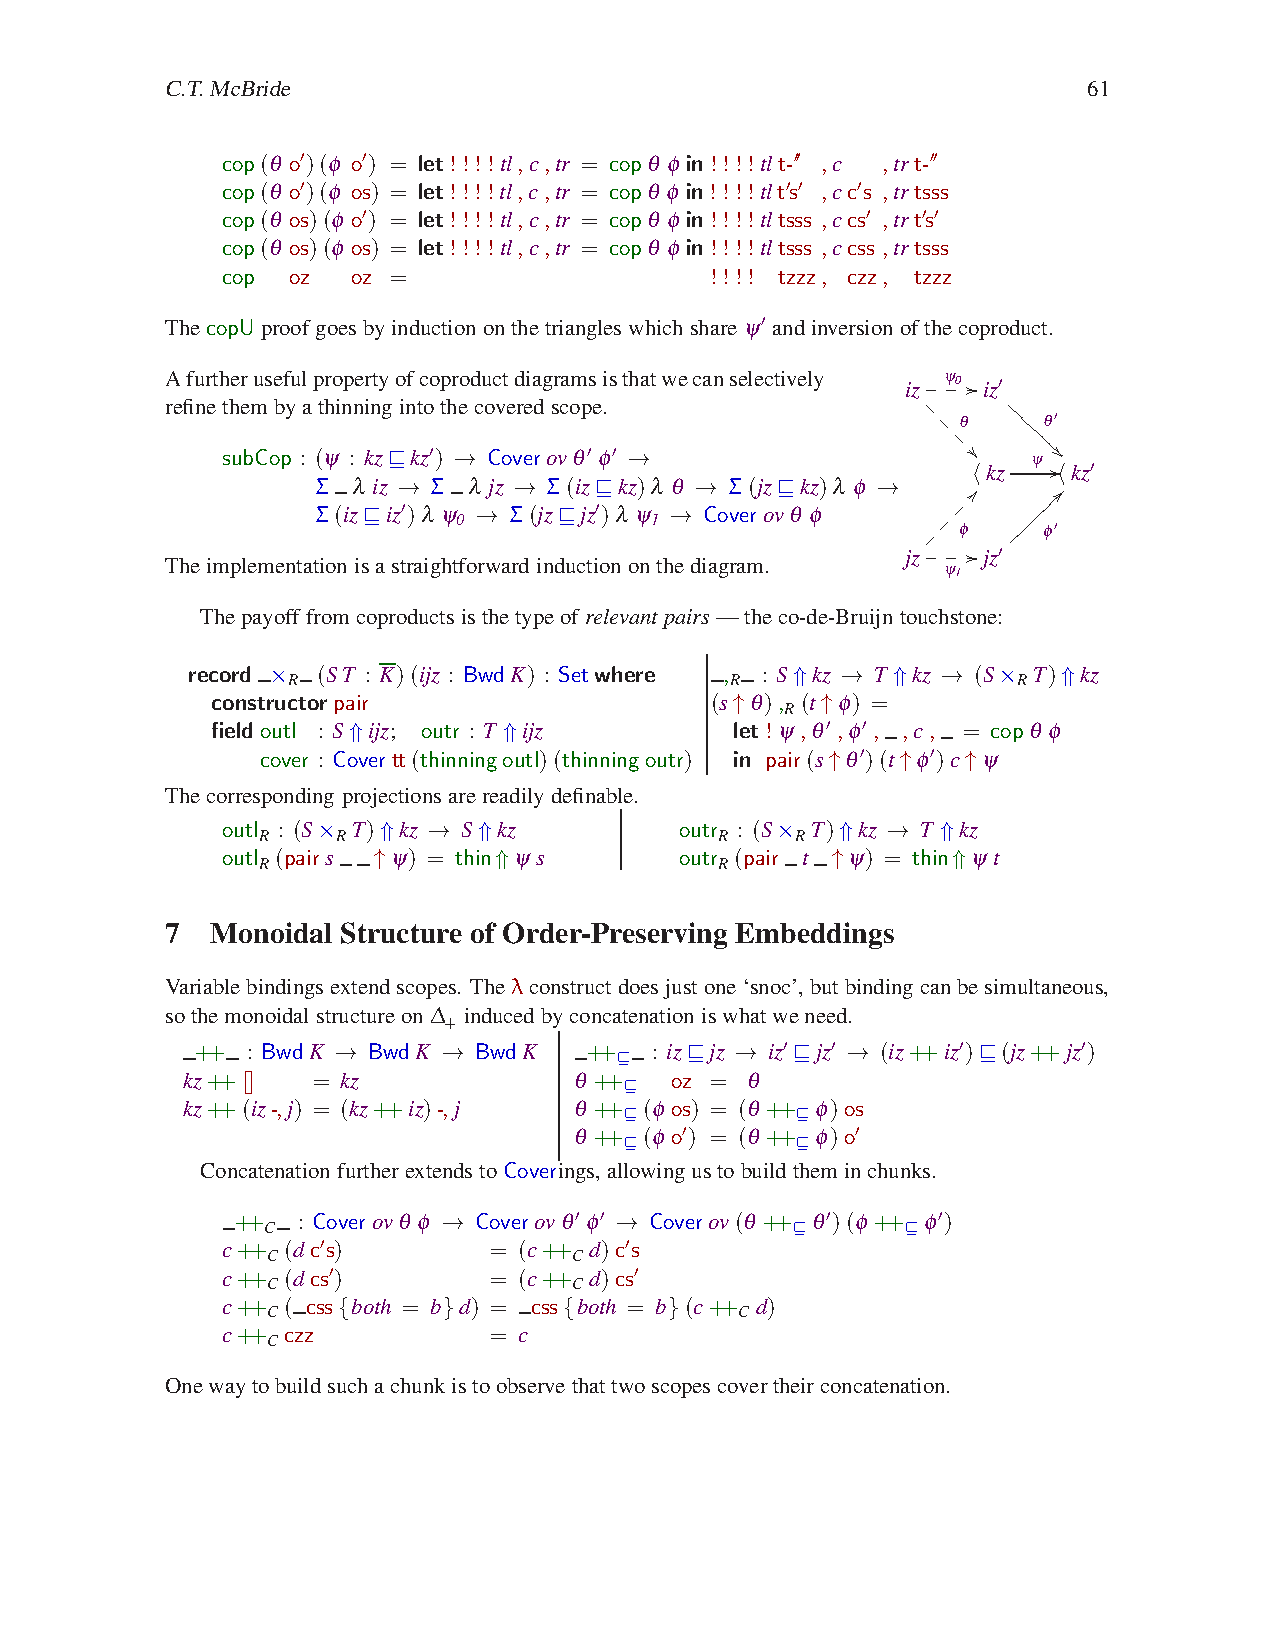
\includegraphics[height=1.15\textheight]{egtbs-9.pdf}
    \end{column}
  \end{columns}
\end{frame}

\begin{frame}
  \frametitle{Using co-De Bruijn is not hard, category theory is!}
    \begin{AgdaSuppressSpace}
      \begin{code}[hide]%
\>[0]\AgdaKeyword{module}\AgdaSpace{}%
\AgdaModule{codebruijn}\AgdaSpace{}%
\AgdaKeyword{where}\<%
\\
\>[0]\AgdaKeyword{open}\AgdaSpace{}%
\AgdaKeyword{import}\AgdaSpace{}%
\AgdaModule{Data.Nat}\AgdaSpace{}%
\AgdaKeyword{using}\AgdaSpace{}%
\AgdaSymbol{(}\AgdaDatatype{ℕ}\AgdaSymbol{;}\AgdaSpace{}%
\AgdaInductiveConstructor{zero}\AgdaSymbol{;}\AgdaSpace{}%
\AgdaInductiveConstructor{suc}\AgdaSymbol{)}\<%
\\
\>[0]\AgdaKeyword{variable}\<%
\\
\>[0][@{}l@{\AgdaIndent{0}}]%
\>[4]\AgdaGeneralizable{k}\AgdaSpace{}%
\AgdaGeneralizable{l}\AgdaSpace{}%
\AgdaGeneralizable{m}\AgdaSpace{}%
\AgdaGeneralizable{n}\AgdaSpace{}%
\AgdaSymbol{:}\AgdaSpace{}%
\AgdaDatatype{ℕ}\<%
\end{code}
\begin{code}%
\>[0]\AgdaKeyword{data}\AgdaSpace{}%
\AgdaDatatype{Cov}\AgdaSpace{}%
\AgdaSymbol{:}\AgdaSpace{}%
\AgdaSymbol{(}\AgdaBound{k}\AgdaSpace{}%
\AgdaBound{l}\AgdaSpace{}%
\AgdaBound{m}\AgdaSpace{}%
\AgdaSymbol{:}\AgdaSpace{}%
\AgdaDatatype{ℕ}\AgdaSymbol{)}\AgdaSpace{}%
\AgdaSymbol{→}\AgdaSpace{}%
\AgdaPrimitive{Set}\AgdaSpace{}%
\AgdaKeyword{where}\<%
\\
\>[0][@{}l@{\AgdaIndent{0}}]%
\>[4]\AgdaInductiveConstructor{⋅}\AgdaSpace{}%
\AgdaSymbol{:}%
\>[20]\AgdaDatatype{Cov}%
\>[29]\AgdaNumber{0}%
\>[37]\AgdaNumber{0}%
\>[45]\AgdaNumber{0}\<%
\\
%
\>[4]\AgdaInductiveConstructor{L}\AgdaSpace{}%
\AgdaSymbol{:}\AgdaSpace{}%
\AgdaDatatype{Cov}\AgdaSpace{}%
\AgdaGeneralizable{k}\AgdaSpace{}%
\AgdaGeneralizable{l}\AgdaSpace{}%
\AgdaGeneralizable{m}\AgdaSpace{}%
\AgdaSymbol{→}\AgdaSpace{}%
\AgdaDatatype{Cov}\AgdaSpace{}%
\AgdaSymbol{(}\AgdaInductiveConstructor{suc}\AgdaSpace{}%
\AgdaGeneralizable{k}\AgdaSymbol{)}%
\>[37]\AgdaGeneralizable{l}%
\>[40]\AgdaSymbol{(}\AgdaInductiveConstructor{suc}\AgdaSpace{}%
\AgdaGeneralizable{m}\AgdaSymbol{)}\<%
\\
%
\>[4]\AgdaInductiveConstructor{R}\AgdaSpace{}%
\AgdaSymbol{:}\AgdaSpace{}%
\AgdaDatatype{Cov}\AgdaSpace{}%
\AgdaGeneralizable{k}\AgdaSpace{}%
\AgdaGeneralizable{l}\AgdaSpace{}%
\AgdaGeneralizable{m}\AgdaSpace{}%
\AgdaSymbol{→}\AgdaSpace{}%
\AgdaDatatype{Cov}%
\>[29]\AgdaGeneralizable{k}%
\>[32]\AgdaSymbol{(}\AgdaInductiveConstructor{suc}\AgdaSpace{}%
\AgdaGeneralizable{l}\AgdaSymbol{)}\AgdaSpace{}%
\AgdaSymbol{(}\AgdaInductiveConstructor{suc}\AgdaSpace{}%
\AgdaGeneralizable{m}\AgdaSymbol{)}\<%
\\
%
\>[4]\AgdaInductiveConstructor{B}\AgdaSpace{}%
\AgdaSymbol{:}\AgdaSpace{}%
\AgdaDatatype{Cov}\AgdaSpace{}%
\AgdaGeneralizable{k}\AgdaSpace{}%
\AgdaGeneralizable{l}\AgdaSpace{}%
\AgdaGeneralizable{m}\AgdaSpace{}%
\AgdaSymbol{→}\AgdaSpace{}%
\AgdaDatatype{Cov}\AgdaSpace{}%
\AgdaSymbol{(}\AgdaInductiveConstructor{suc}\AgdaSpace{}%
\AgdaGeneralizable{k}\AgdaSymbol{)}\AgdaSpace{}%
\AgdaSymbol{(}\AgdaInductiveConstructor{suc}\AgdaSpace{}%
\AgdaGeneralizable{l}\AgdaSymbol{)}\AgdaSpace{}%
\AgdaSymbol{(}\AgdaInductiveConstructor{suc}\AgdaSpace{}%
\AgdaGeneralizable{m}\AgdaSymbol{)}\<%
\\
%
\\[\AgdaEmptyExtraSkip]%
\>[0]\AgdaKeyword{data}\AgdaSpace{}%
\AgdaDatatype{Term}\AgdaSpace{}%
\AgdaSymbol{:}\AgdaSpace{}%
\AgdaDatatype{ℕ}\AgdaSpace{}%
\AgdaSymbol{→}\AgdaSpace{}%
\AgdaPrimitive{Set}\AgdaSpace{}%
\AgdaKeyword{where}\<%
\\
\>[0][@{}l@{\AgdaIndent{0}}]%
\>[4]\AgdaInductiveConstructor{\#}%
\>[12]\AgdaSymbol{:}\AgdaSpace{}%
\AgdaDatatype{Term}\AgdaSpace{}%
\AgdaNumber{1}\<%
\\
%
\>[4]\AgdaInductiveConstructor{ƛ}%
\>[12]\AgdaSymbol{:}\AgdaSpace{}%
\AgdaDatatype{Term}\AgdaSpace{}%
\AgdaSymbol{(}\AgdaInductiveConstructor{suc}\AgdaSpace{}%
\AgdaGeneralizable{n}\AgdaSymbol{)}\AgdaSpace{}%
\AgdaSymbol{→}\AgdaSpace{}%
\AgdaDatatype{Term}\AgdaSpace{}%
\AgdaGeneralizable{n}\<%
\\
%
\>[4]\AgdaOperator{\AgdaInductiveConstructor{\AgdaUnderscore{}\$[\AgdaUnderscore{}]\AgdaUnderscore{}}}%
\>[12]\AgdaSymbol{:}\AgdaSpace{}%
\AgdaDatatype{Term}\AgdaSpace{}%
\AgdaGeneralizable{k}\AgdaSpace{}%
\AgdaSymbol{→}\AgdaSpace{}%
\AgdaDatatype{Cov}\AgdaSpace{}%
\AgdaGeneralizable{k}\AgdaSpace{}%
\AgdaGeneralizable{l}\AgdaSpace{}%
\AgdaGeneralizable{m}\AgdaSpace{}%
\AgdaSymbol{→}\AgdaSpace{}%
\AgdaDatatype{Term}\AgdaSpace{}%
\AgdaGeneralizable{l}\AgdaSpace{}%
\AgdaSymbol{→}\AgdaSpace{}%
\AgdaDatatype{Term}\AgdaSpace{}%
\AgdaGeneralizable{m}\<%
\\
\>[0]\<%
\\
\>[0]\AgdaFunction{\AgdaUnderscore{}}\AgdaSpace{}%
\AgdaSymbol{=}\AgdaSpace{}%
\AgdaInductiveConstructor{ƛ}\AgdaSpace{}%
\AgdaSymbol{(}\AgdaInductiveConstructor{ƛ}\AgdaSpace{}%
\AgdaSymbol{(}\AgdaInductiveConstructor{ƛ}\AgdaSpace{}%
\AgdaSymbol{((}\AgdaInductiveConstructor{\#}\AgdaSpace{}%
\AgdaOperator{\AgdaInductiveConstructor{\$[}}\AgdaSpace{}%
\AgdaInductiveConstructor{L}\AgdaSpace{}%
\AgdaSymbol{(}\AgdaInductiveConstructor{R}\AgdaSpace{}%
\AgdaInductiveConstructor{⋅}\AgdaSymbol{)}\AgdaSpace{}%
\AgdaOperator{\AgdaInductiveConstructor{]}}\AgdaSpace{}%
\AgdaInductiveConstructor{\#}\AgdaSymbol{)}\AgdaSpace{}%
\AgdaOperator{\AgdaInductiveConstructor{\$[}}\AgdaSpace{}%
\AgdaInductiveConstructor{L}\AgdaSpace{}%
\AgdaSymbol{(}\AgdaInductiveConstructor{R}\AgdaSpace{}%
\AgdaSymbol{(}\AgdaInductiveConstructor{B}\AgdaSpace{}%
\AgdaInductiveConstructor{⋅}\AgdaSymbol{))}\AgdaSpace{}%
\AgdaOperator{\AgdaInductiveConstructor{]}}\AgdaSpace{}%
\AgdaSymbol{(}\AgdaInductiveConstructor{\#}\AgdaSpace{}%
\AgdaOperator{\AgdaInductiveConstructor{\$[}}\AgdaSpace{}%
\AgdaInductiveConstructor{L}\AgdaSpace{}%
\AgdaSymbol{(}\AgdaInductiveConstructor{R}\AgdaSpace{}%
\AgdaInductiveConstructor{⋅}\AgdaSymbol{)}\AgdaSpace{}%
\AgdaOperator{\AgdaInductiveConstructor{]}}\AgdaSpace{}%
\AgdaInductiveConstructor{\#}\AgdaSymbol{))))}\<%
\end{code}
    \end{AgdaSupressSpace}
\end{frame}

\subsection{References}
\begin{frame}[fragile]
  \frametitle{References}
  \nocite{catsandtypes}
  \printbibliography{}
\end{frame}

\end{document}